%*****************************************
\chapter{Lab 02: Frequencies}\label{ch:lab02}
%*****************************************
%\setcounter{figure}{10}
%\NoCaseChange{Homo Sapiens}

\section{Introduction}

Nominal and Ordinal data items are normally reported in frequency tables where the counts for a particular item are displayed and this lab explores frequency tables and visualization techniques that are used to make frequencies easier to comprehend.

\section{Discussion}

\subsection{Frequency Tables}

A frequency table simply lists a count of the number of times that some nominal or ordinal data item appears in a dataset. These types of tables are common around election time when polls report the number of people who voted for or against some proposition. As an example, here is a frequency table for the passenger rating in the \textit{cars} dataset.

\begin{figure}[H]
  \begin{center}
    \fbox{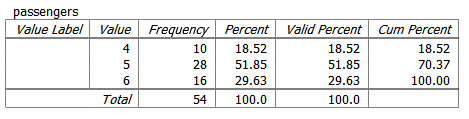
\includegraphics[]{gfx/lab02_fig01}}
    \caption{Number of Passengers Per Car}
    \label{lab02_fig01}    
  \end{center}
\end{figure}

The above table shows that $ 10 $ cars in the dataset were rated for four passengers, $ 28 $ for five passengers, and $ 16 $ for six passengers, for a total of $ 54 $ rated cars. The table also shows the various row percentages so the researcher could report that $ 18.5\% $ of the cars were rated for four passengers. The ``Valid Percent'' column indicates the percentage of cases when missing cases are removed. In this dataset there were no missing cases so the Valid Percent column is the same as the ``Percent'' column.

A second example of a frequency table was created from the \textit{email} dataset. This frequency table shows the number of images that were attached to messages.

\begin{figure}[H]
  \begin{center}
    \fbox{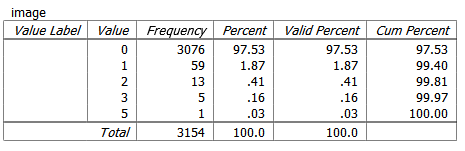
\includegraphics[]{gfx/lab02_fig02}}
    \caption{Images Per Message}
    \label{lab02_fig02}
  \end{center}
\end{figure}

Figure \ref{lab02_fig02} shows that $ 97.5\% $ of $ 3154 $ email messages contained no images while a small number of messages contained one or more images.

Frequency tables are only useful for nominal or ordinal data-type items. To illustrate why this is true, imagine creating a survey for all of the students at the University of Arizona and including ``age'' (interval-type data) as one of the survey questions. Attempting to create a frequency table for the ages of the respondents would have, potentially, more than $ 65 $ rows since student ages would range from about $ 15 $ to more than $ 80 $ and each row would report the number of students for that age. While a frequency table that large could be created it would have so many rows that it would be virtually unusable.

\subsection{Visualizing Frequency}

There are many ways to visualize frequency data and people often find that graphs aid in comprehension. This lab introduces the visualization tools available in \acs{PSPP}.

\subsubsection{Histogram}

A histogram is a graph that shows how often various responses were selected on a survey. These are often presented as a graphic representation of the statistical data found in a frequency table in order to aid in understanding. Histograms are only used for data that are interval or ratio in nature, for example, age or height. 

As an example of a histogram, Figure \ref{lab02_fig07} shows the mother's age from the \textit{births} dataset.

\begin{figure}[H]
  \begin{center}
    \fbox{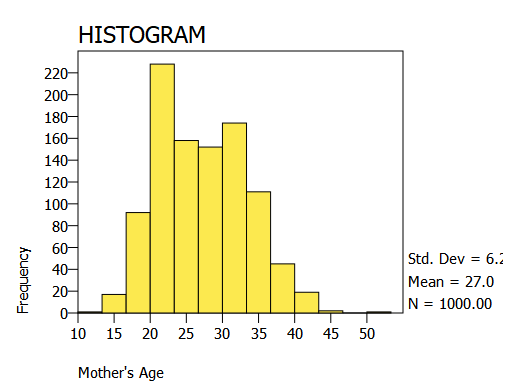
\includegraphics[width=0.95\linewidth]{gfx/lab02_fig07}}
    \caption{Histogram of Mother's Age}
    \label{lab02_fig07}
  \end{center}
\end{figure}

Notice that there is not a separate bar for each age; rather, \acs{PSPP} has clustered three years into the same bar. Thus, there is a bar that combines $ 20 $-$ 22 $ and not separate bars for $ 20 $, $ 21 $, and $ 22 $.

As another example, Figure \ref{lab02_fig08} shows a histogram for baby's weight from the \textit{births} dataset.\footnote{Using a histogram aids a researcher in determining if a dataset is normally distributed and skewed. Figure \ref{lab02_fig08} shows a normally distributed dataset since there is a clear peak in the middle trailing off on both sides. It also shows a negative skew since the tails on the left side of the peak are longer. Lab \ref{int:normal_distribution} on page \pageref{int:normal_distribution} discusses the shape of a normal distribution.}

\begin{figure}[H]
  \begin{center}
    \fbox{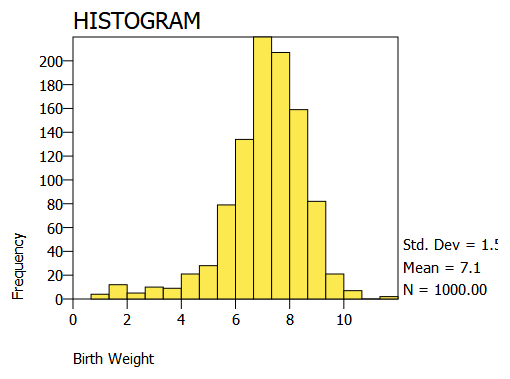
\includegraphics[width=0.95\linewidth]{gfx/lab02_fig08}}
    \caption{Histogram of Baby's Weight}
    \label{lab02_fig08}
  \end{center}
\end{figure}

As in Figure \ref{lab02_fig07}, each bar represents a range of weights so any weight between $ 6 $ and $ 6.33 $ pounds is clustered in a single bar.

\subsubsection{Bar Chart} A bar chart is used to display the frequency count for ordinal or nominal data. There are technical differences between a bar chart and a histogram but for the purposes of this lab manual they can be considered identical displays for different types of data. Figure \ref{lab02_fig09} is a bar chart showing the prevalence of various drive trains in the \textit{cars} dataset.

\begin{figure}[H]
  \begin{center}
    \fbox{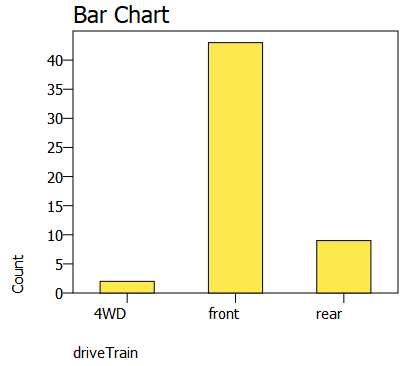
\includegraphics[width=.75\linewidth]{gfx/lab02_fig09}}
    \caption{Prevelance of Types of Drive Trains}
    \label{lab02_fig09}
  \end{center}
\end{figure}

Figure \ref{lab02_fig10} shows the maturity level of the mothers in the \textit{births} dataset and unsurprisingly indicates that most mothers are younger.

\begin{figure}[H]
  \begin{center}
    \fbox{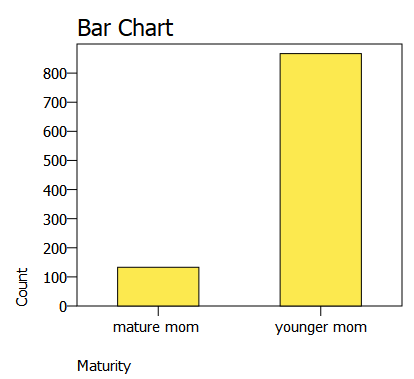
\includegraphics[width=.75\linewidth]{gfx/lab02_fig10}}
    \caption{Maturity of Mothers}
    \label{lab02_fig10}
  \end{center}
\end{figure}

\subsubsection{Clustered Bar Chart} A clustered bar chart displays two or more variables and is used to display ordinal or nominal data. In general, clustered bar charts can be difficult to interpret and should be avoided. Figure \ref{lab02_fig11} is a clustered bar chart that shows the incidence of premature births by the mother's smoking habit in the \textit{births} dataset.

\begin{figure}[H]
  \begin{center}
    \fbox{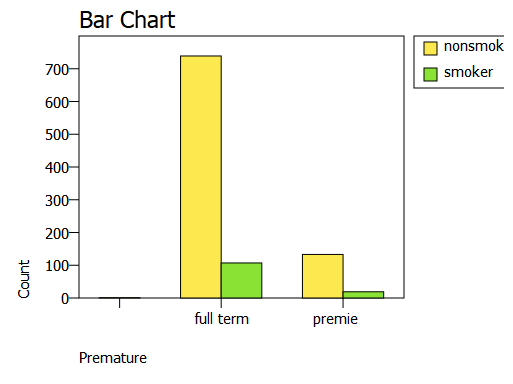
\includegraphics[width=0.95\linewidth]{gfx/lab02_fig11}}
    \caption{Permature Births By Smoking Habit}
    \label{lab02_fig11}
  \end{center}
\end{figure}

Figure \ref{lab02_fig12} illustrates the problem with a clustered bar chart. This is a chart that shows the number of passengers for each type of car in the \textit{cars} dataset. Notice that no large cars have four or five passengers and no small cars have  six passengers so those bars are missing and that can make the chart difficult to interpret.

\begin{figure}[H]
  \begin{center}
    \fbox{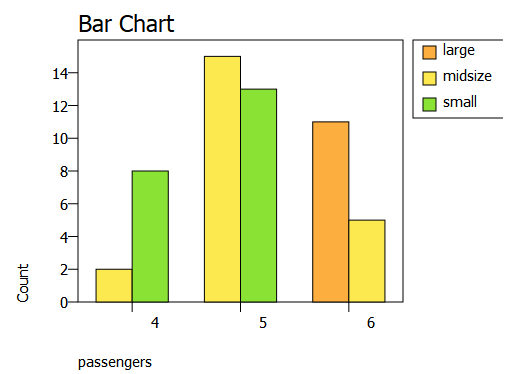
\includegraphics[width=0.95\linewidth]{gfx/lab02_fig12}}
    \caption{Number of Passengers By Car Type}
    \label{lab02_fig12}
  \end{center}
\end{figure}

\subsubsection{Pie Chart} A pie chart is commonly used to display nominal or ordinal data; however, pie charts are notoriously difficult to understand, especially if the writer uses some sort of $ 3 $-D effect or ``exploded'' slices. The human brain seems able to easily compare the \textit{heights} of two or more bars, as in histograms and bar charts, but the \textit{areas} of two or more slices of a pie chart are difficult to compare. For this reason, pie charts should be avoided in research reports. If they are used at all, they should only illustrate one slice's relationship to the whole, not comparing one slice to another; and no more than four or five slices should be presented on one chart.

Figure \ref{lab02_fig13} shows the types of numbers found in messages in the \textit{email} dataset. This pie chart is easy to interpret since there are only three slices and each slice is easy to compare to the whole.

\begin{figure}[H]
  \begin{center}
    \fbox{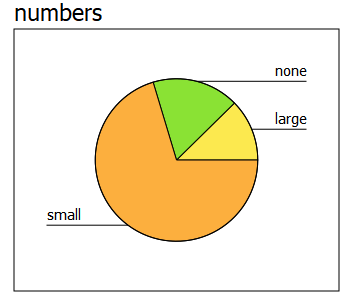
\includegraphics[width=0.7\linewidth]{gfx/lab02_fig13}}
    \caption{Types of Numbers in Email Messages}
    \label{lab02_fig13}
  \end{center}
\end{figure}

As an extreme example of a poorly used pie chart, consider Figure \ref{lab02_fig14}. Even ignoring the problem of the numbered labels overlapping, making them impossible to read, the slices are so numerous and small that it is impossible to differentiate between them. For example, the ``one'' and ``two'' slices are impossible to compare. For this pie chart, about all that can be stated is that most email messages have zero dollar signs.

\begin{figure}[H]
  \begin{center}
    \fbox{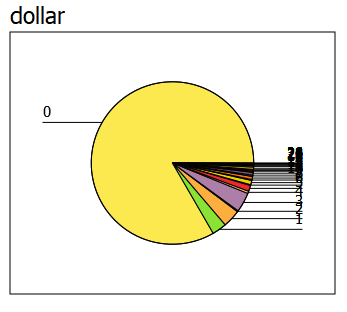
\includegraphics[width=0.7\linewidth]{gfx/lab02_fig14}}
    \caption{Number of Times a Dollar Sign Used in Email Messages}
    \label{lab02_fig14}
  \end{center}
\end{figure}

\section{Procedure}

\subsection{Frequency Table}

Start \acs{PSPP} and open the \textit{email} dataset, then:

\begin{enumerate}
  \item Click \textsc{\fbox{Analyze $ \rightarrow $ Descriptive Statistics $ \rightarrow $ Frequencies}}
  \item Click the word \textit{format} in the left column and then click the right-arrow button near the center of the window to move \textit{format} to the ``Variables'' box on the right side of the window. (Alternatively, double-click the word \textit{format} in the left column to move it to the ``Variables'' box.)
  \item Uncheck all ``Statistics'' options in the lower-right box.
  \item It is safe to explore the ``Charts'' and ``Frequency Tables'' options but do not select any of those options, they will be demonstrated later.
  \item Click \fbox{OK} to generate the frequency table.
\end{enumerate}

\begin{figure}[H]
  \begin{center}
    \fbox{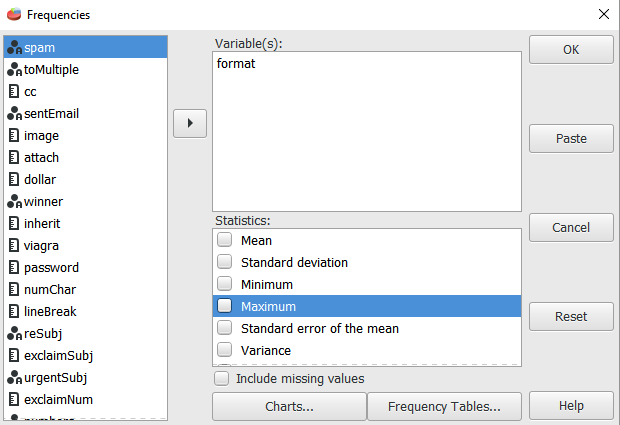
\includegraphics[width=\linewidth]{gfx/lab02_fig03}}
    \caption{Generating a Frequency Table}
    \label{lab02_fig03}    
  \end{center}
\end{figure}

\begin{figure}[H]
  \begin{center}
    \fbox{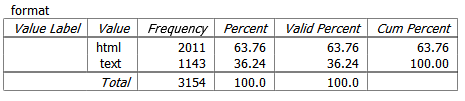
\includegraphics[width=\linewidth]{gfx/lab02_fig04}}
    \caption{Email Format Frequency Table}
    \label{lab02_fig04}    
  \end{center}
\end{figure}

\subsubsection{Activity 1: Frequency Table} \label{lab02_act01}

Using the \textit{births} dataset, produce a frequency table for \textit{gender}.

\subsubsection{Activity 2: Frequency Table} \label{lab02_act02}

Using the \textit{cafe} dataset, produce a frequency table for \textit{meal}.

\subsection{Histogram}

Start \acs{PSPP} and open the \textit{bdims} dataset, then:

\begin{enumerate}
  \item Click \textsc{\fbox{Graphs $ \rightarrow $ Histogram}}\footnote{Histograms can also be specified as an optional chart when creating a Frequency Table.}
  \item Click the word \textit{age} in the left column and then click the right-arrow button near the center of the window to move \textit{age} to the ``Variable'' box on the right side of the window. (Alternatively, double-click the word \textit{age} in the left column to move it to the ``Variable'' box.)
  \item Click \fbox{OK} to generate the histogram.
\end{enumerate}

\begin{figure}[H]
  \begin{center}
    \fbox{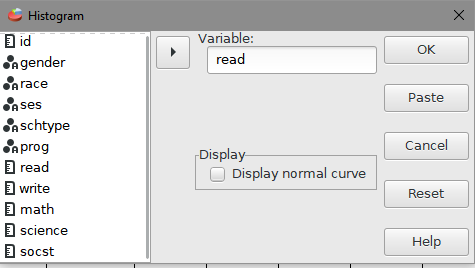
\includegraphics[width=\linewidth]{gfx/lab02_fig15}}
    \caption{Generating a Histogram}
    \label{lab02_fig15}
  \end{center}
\end{figure}

\begin{figure}[H]
  \begin{center}
    \fbox{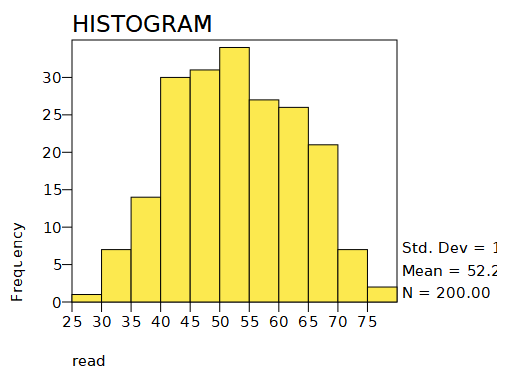
\includegraphics[width=\linewidth]{gfx/lab02_fig16}}
    \caption{Age Histogram}
    \label{lab02_fig16}
  \end{center}
\end{figure}

\subsubsection{Activity 3: Histogram} \label{lab02_act03}

Using the \textit{email} dataset, produce a histogram for \textit{numChar} (the number of characters, in thousands, in the email message).

\subsubsection{Activity 4: Histogram} \label{lab02_act04}

Using the \textit{cafe} dataset, produce a histogram for \textit{age}.

\subsection{Bar Chart}

Start \acs{PSPP} and open the \textit{cars} dataset, then:

\begin{enumerate}
  \item Click \textsc{\fbox{Graphs $ \rightarrow $ Barchart}}\footnote{Bar charts can also be specified as an optional chart when creating a Frequency Table.}
  \item Click the word \textit{passengers} in the left column and then click the right-arrow button near the center of the window to move \textit{passengers} to the ``Category Axis'' box on the right side of the window.
  \item Click \fbox{OK} to generate the bar chart.
\end{enumerate}

\begin{figure}[H]
  \begin{center}
    \fbox{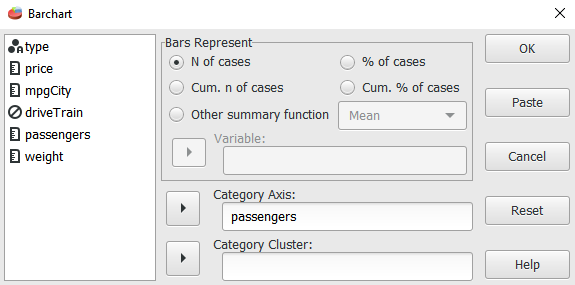
\includegraphics[width=\linewidth]{gfx/lab02_fig17}}
    \caption{Generating a Bar Chart}
    \label{lab02_fig17}
  \end{center}
\end{figure}

\begin{figure}[H]
  \begin{center}
    \fbox{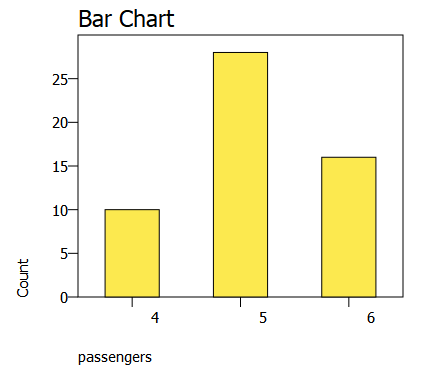
\includegraphics[width=\linewidth]{gfx/lab02_fig18}}
    \caption{Passengers Bar Chart}
    \label{lab02_fig18}
  \end{center}
\end{figure}

\subsubsection{Activity 5: Bar Chart} \label{lab02_act05}

Using the \textit{email} dataset, produce a bar chart for \textit{numbers}.

\subsubsection{Activity 6: Bar Chart} \label{lab02_act06}

Using the \textit{cafe} dataset, produce a barchart for \textit{meal}.

\subsection{Clustered Bar Chart}

Start \acs{PSPP} and open the \textit{births} dataset, then:

\begin{enumerate}
  \item Click \textsc{\fbox{Graphs $ \rightarrow $ Barchart}}
  \item Click the word \textit{premie} in the left column and then click the right-arrow button near the center of the window to move \textit{premie} to the ``Category Axis'' box on the right side of the window.
  \item Click the word \textit{mature} in the left column and then click the right-arrow button near the bottom of the window to move \textit{mature} to the ``Category Cluster'' box on the right side of the window.
  \item Click \fbox{OK} to generate the bar chart.
\end{enumerate}

\begin{figure}[H]
  \begin{center}
    \fbox{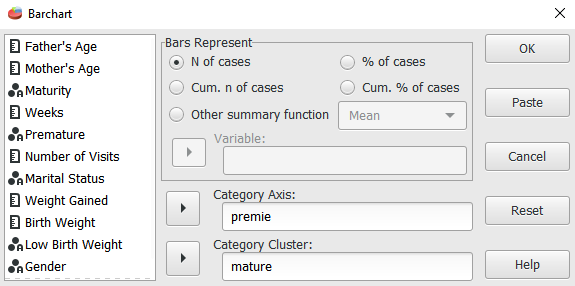
\includegraphics[width=\linewidth]{gfx/lab02_fig19}}
    \caption{Generating a Clustered Bar Chart}
    \label{lab02_fig19}
  \end{center}
\end{figure}

\begin{figure}[H]
  \begin{center}
    \fbox{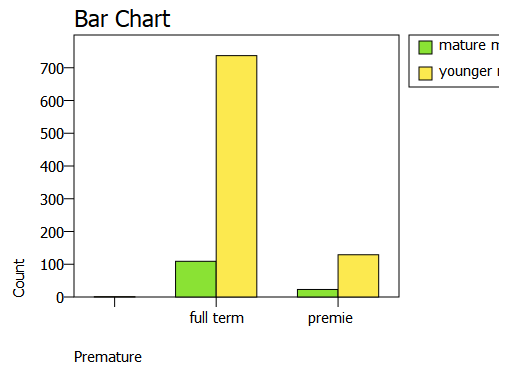
\includegraphics[width=\linewidth]{gfx/lab02_fig20}}
    \caption{Clustered Bar Chart}
    \label{lab02_fig20}
  \end{center}
\end{figure}

\subsubsection{Activity 7: Clustered Bar Chart} \label{lab02_act07}

Using the \textit{cars} dataset, produce a clustered bar chart using \textit{drive train} by \textit{type}.

\subsubsection{Activity 8: Clustered Bar Chart} \label{lab02_act08}

Using the \textit{cafe} dataset, produce a clustered bar chart for \textit{meal} by \textit{sex}.

\subsection{Pie Chart}

Start \acs{PSPP} and open the \textit{cars} dataset, then:

\begin{enumerate}
  \item Click \textsc{\fbox{Analyze $ \rightarrow $ Descriptive Statistics $ \rightarrow $ Frequencies}}
  \item Click the word \textit{driveTrain} in the left column and then click the right-arrow button near the center of the window to move \textit{driveTrain} to the ``Variable(s)'' box on the right side of the window.
  \item Uncheck all of the ``Statistics'' boxes in the lower-right text box.
  \item Click \fbox{Charts} to open the charts options window.
  \item Select ``Draw pie charts''
  \item Click \fbox{Continue}
  \item Click \fbox{OK} to generate the pie chart.
\end{enumerate}

\begin{figure}[H]
  \begin{center}
    \fbox{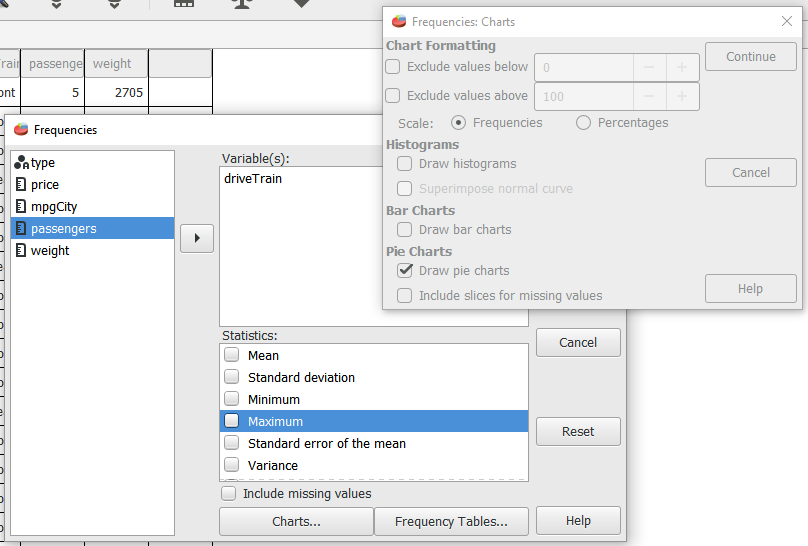
\includegraphics[width=\linewidth]{gfx/lab02_fig21}}
    \caption{Generating a Pie Chart}
    \label{lab02_fig21}
  \end{center}
\end{figure}

\begin{figure}[H]
  \begin{center}
    \fbox{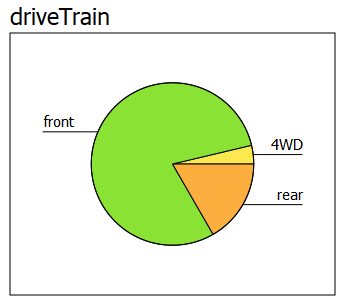
\includegraphics[width=\linewidth]{gfx/lab02_fig22}}
    \caption{Pie Chart}
    \label{lab02_fig22}
  \end{center}
\end{figure}

\subsubsection{Activity 9: Pie Chart} \label{lab02_act09}

Using the \textit{cars} dataset, produce a pie using \textit{passengers}.

\subsubsection{Activity 10: Pie Chart} \label{lab02_act10}

Using the \textit{cafe} dataset, produce a pie chart for \textit{meal} by \textit{sex}.

\section{Deliverable}

Complete the following activities in this lab:

\rowcolors{1}{gray!25}{}
\begin{center}
  \begin{tabular}{lll}
    \hline 
    \textbf{Number} & \textbf{Name} & \textbf{Page} \\ 
    \hline 
    \ref{lab02_act01} & \nameref{lab02_act01} & \pageref{lab02_act01} \\ 
    \ref{lab02_act02} & \nameref{lab02_act02} & \pageref{lab02_act02} \\ 
    \ref{lab02_act03} & \nameref{lab02_act03} & \pageref{lab02_act03} \\ 
    \ref{lab02_act04} & \nameref{lab02_act04} & \pageref{lab02_act04} \\ 
    \ref{lab02_act05} & \nameref{lab02_act05} & \pageref{lab02_act05} \\ 
    \ref{lab02_act06} & \nameref{lab02_act06} & \pageref{lab02_act06} \\ 
    \ref{lab02_act07} & \nameref{lab02_act07} & \pageref{lab02_act07} \\ 
    \ref{lab02_act08} & \nameref{lab02_act08} & \pageref{lab02_act08} \\ 
    \ref{lab02_act09} & \nameref{lab02_act09} & \pageref{lab02_act09} \\ 
    \ref{lab02_act10} & \nameref{lab02_act10} & \pageref{lab02_act10} \\ 
    \hline 
  \end{tabular} 
\end{center}

Consolidate the responses for all activities into a single document and submit that document for grading.


